%% LyX 2.3.6.1 created this file.  For more info, see http://www.lyx.org/.
%% Do not edit unless you really know what you are doing.
\documentclass[english]{article}
\usepackage[T1]{fontenc}
\usepackage[latin9]{inputenc}
\usepackage{array}
\usepackage{booktabs}
\usepackage{url}
\usepackage{multirow}
\usepackage{graphicx}

\makeatletter

%%%%%%%%%%%%%%%%%%%%%%%%%%%%%% LyX specific LaTeX commands.
%% Because html converters don't know tabularnewline
\providecommand{\tabularnewline}{\\}
%% A simple dot to overcome graphicx limitations
\newcommand{\lyxdot}{.}


%%%%%%%%%%%%%%%%%%%%%%%%%%%%%% User specified LaTeX commands.
\usepackage {a4wide}

\@ifundefined{showcaptionsetup}{}{%
 \PassOptionsToPackage{caption=false}{subfig}}
\usepackage{subfig}
\makeatother

\usepackage{babel}
\begin{document}
\title{Exploring Dew Computing for distributed inference using real testbeds}
\maketitle
\begin{abstract}
Is Dew computing a competitive resource provider for realtime image
processing scenarios? Today's IoT applications still have a strong
dependency on Cloud resources, platforms and services. Many efforts
consider edge resources as an alternative to long latency cloud resources
in fullfilling IoT workloads but few of these works evaluate the performance
achieved on real testbeds. Moreover, few to none work derive guidelines
to help system designers to consider the usage of  low cost dew computing
hardware such as a Raspberry Pi or nomadic hardware including smartphones
clusters. Given the popularity gained by neural networks such as DNN
and CNN for solving image classification problems, the developement
of libraries like tensorflow which in its lite version allows practitioners
to perform inferences with resource limited hardware, and the strong
relation such inference tasks with many IoT applications that use
images as input, we elaborate a first-cut approach to such a guideline
with data derived from experiments on real test beds. First, we classify
dew computing scenarios based on a multidimensional analysis of stream
workloads with dimensions including data volume generated, data volume
time distribution and processing time required per data unit.
\end{abstract}

\section{Introduction}

As formally described in~\cite{gusev2018formal}, Dew computing has
two modes of operation, local mode and global mode. In local mode,
services are provided with resources within a local scope to where
computing needs belong, in other words, using resources that can be
accessed within the local perimeter of a local area network. On the
contrast, global mode involves communication with Cloud server. In
this work, we concentrate on evaluating cloud-independant capabilities,
i.e., ability to render service offline. We do this by measuring ability
of dew computing instances to accomplish with different workloads
by exclusively relying on its local operation mode capabilities.
\begin{itemize}
\item \textit{Presentar AI en el edge resaltando aspectos claves (posibilidad
de ejecutar AI acudiendo lo menos posible al poder de c�mputo de la
nube, privacidad de datos). Desarrollar estudio de Pablo sobre benchmarking
en m�viles individuales.}
\item \textit{Sin entrar en profundidad, mencionar trabajos que muestren
el valor de realizar ``Distributed inference'' en el edge. Introducir
el concepto de Dew Computing como paradigma que aprovecha la capacidad
de c�mputo para realizar AI, no considerando capacidad de smartphones
de forma aislada sin� planteando el aprovechamiento de clusters de
smartphones.}
\item \textit{Terminar intro indicando qu� se va a hacer relacionado a ``Distributed
Inference'' en el edge.}
\end{itemize}

\section{Related works}

In this section we differentiate and objectively discuss efforts in
the fields of distributed inference research considering mobile devices
as main computing power nodes. Such differentiation allow the reader
to rapidly contextualize the contribution of this work.
\begin{itemize}
\item \textit{Discutir trabajos sobre distributed inference. Ejes de discuci�n
que ser�an necesario incluir: }
\begin{itemize}
\item \textit{Ejecuci�n de la inferencia: �Ente qu� capas de nodos se realiza
la distribuci�n de la inferencia (esto seguramente fuerce a tomar
definiciones sobre edge, fog, cloud)? �s�lo Edge?, �s�lo Cloud? �Edge
y Cloud? �Dew?}
\item \textit{Tipo de evaluaci�n: �sobre ambientes reales?, �sobre ambientes
simulados?}
\end{itemize}
\item \textit{Converger a que no hay trabajos que muestren emp�ricamente
lo que un grupo de dispositivos puede ofrecer en t�rminos de ``Distributed
inference'' capability.}
\end{itemize}

\section{Approach \& assumptions}
\begin{itemize}
\item \textit{Describir de forma gen�rica la descomposici�n de una arquitectura
de procesamiento de un ambiente dew, mencionando las funciones de
los componentes estableciendo un correspondencia con los siguientes
roles:}
\begin{itemize}
\item \textit{rol sensador de datos (nodo que a partir de una orden recibida
comienza a enviar datos a un nodo concentrador de dichos datos)}
\item \textit{rol concentrador de datos (buffering, data ingestion) (este
rol tambi�n se podr�a ver de reemplazar/asociar a la idea de una tarea
de sensado del contexto que dispara o no la toma de datos)}
\item \textit{rol pre-procesador de datos (conversi�n de datos de entrada
en tareas AI, se puede asociar con conceptos de stream processing
\--fixed windows, overlapping windows, session windows\--.)}
\item \textit{rol ejecutor de tareas AI}
\end{itemize}
\item \textit{Mostrar instanciaciones: una donde todos los roles sean asignados
a una SBC y otra donde la SBC funcione como concentrador y preprocesador
de datos mientras que el cluster de smartphones como ejecutores.}
\item Idear taxonom�a de escenarios donde sea suficiente/necesario hacer
uso de m�s recursos del edge relacion�ndolo con caracter�sticas de
aplicaciones
\end{itemize}

\section{Empirical evaluation}
\begin{itemize}
\item \textit{Contar el dise�o de experimentos y lo que se busca evaluar
mencionando al mismo tiempo las m�tricas que se utilizar�n para realizar
la evaluaci�n.}
\end{itemize}
In this section we present the results of empirical evaluations of
the computing power of a collaborative execution scheme composed by
mobile devices in the proximity of a wireless LAN. We compare the
performance to edge nodes of type SBC.

\subsection{Computing Nodes}
\begin{itemize}
\item \textit{Describir los nodos que intervendr�n en la inferencia distribuida
mencionando caracter�sticas de hardware y presentando resultados de
benchmarks.}
\end{itemize}
In this section we describe candidate edge nodes for providing the
required computing power in the Dew computing scenarios aforementioned.
We evaluate tree single board computers (SBC) and five mid-range to
low-end different brands smartphone models. 

\begin{table}
\begin{centering}
\begin{tabular*}{1\textwidth}{@{\extracolsep{\fill}}l>{\raggedright}p{0.14\columnwidth}>{\raggedright}p{0.35\columnwidth}>{\raggedright}p{0.15\columnwidth}>{\raggedright}p{0.1\columnwidth}>{\raggedright}p{0.05\columnwidth}}
\toprule 
\multicolumn{1}{>{\raggedright}p{0.03\columnwidth}}{{\footnotesize{}Edge Node Type}} & {\footnotesize{}Edge Node Model} & {\footnotesize{}Processor} & {\footnotesize{}Conectivity} & {\footnotesize{}RAM} & {\footnotesize{}Price (U\$D)}\tabularnewline
\midrule
\midrule 
\multirow{3}{*}{{\footnotesize{}SBC}} & {\footnotesize{}Raspberry Pi 4} & {\footnotesize{}Quad-core 1.5 GHz ARM Cortex-A72} & {\footnotesize{}Wi-Fi 802.11ac} & {\footnotesize{}4 GB LPDDR4 SDRAM} & {\footnotesize{}55}\tabularnewline
\cmidrule{2-6} \cmidrule{3-6} \cmidrule{4-6} \cmidrule{5-6} \cmidrule{6-6} 
 & {\footnotesize{}Jetson Nano} & {\footnotesize{}Quad-core ARM Cortex-A57 MPCore} & {\footnotesize{}Gigabit Ethernet, M.2 Key E} & {\footnotesize{}4 GB 64-bit LPDDR4} & {\footnotesize{}99}\tabularnewline
\cmidrule{2-6} \cmidrule{3-6} \cmidrule{4-6} \cmidrule{5-6} \cmidrule{6-6} 
 & {\footnotesize{}Gigabyte Brix GB-BRi5H-8250} & {\footnotesize{}Intel Quad core i5-8250U} & {\footnotesize{}IEEE 802.11ac, Dual Band Wi-Fi} & {\footnotesize{}8 GB SO-DIMM DDR4} & {\footnotesize{}750(TBC)}\tabularnewline
\midrule 
\multirow{5}{*}{{\footnotesize{}Smartphone}} & {\footnotesize{}Samsung A02} & {\footnotesize{}Quad-core 1.5 GHz Cortex-A53} & {\footnotesize{}Wi-Fi 802.11 b/g/n} & {\footnotesize{}2 GB} & {\footnotesize{}116}\tabularnewline
\cmidrule{2-6} \cmidrule{3-6} \cmidrule{4-6} \cmidrule{5-6} \cmidrule{6-6} 
 & {\footnotesize{}Motorola Moto G6} & {\footnotesize{}Octa-core 1.8 GHz Cortex-A53} & {\footnotesize{}Wi-Fi 802.11 a/b/g/n} & {\footnotesize{}3 GB} & {\footnotesize{}160}\tabularnewline
\cmidrule{2-6} \cmidrule{3-6} \cmidrule{4-6} \cmidrule{5-6} \cmidrule{6-6} 
 & {\footnotesize{}Samsung A30} & {\footnotesize{}Octa-core (2x1.8 GHz Cortex-A73 \& 6x1.6 GHz Cortex-A53)} & {\footnotesize{}Wi-Fi 802.11 a/b/g/n/ac} & {\footnotesize{}3 GB} & {\footnotesize{}170}\tabularnewline
\cmidrule{2-6} \cmidrule{3-6} \cmidrule{4-6} \cmidrule{5-6} \cmidrule{6-6} 
 & {\footnotesize{}Xiaomi Redmi Note 7} & {\footnotesize{}Octa-core (4x2.2 GHz Kryo 260 Gold \& 4x1.8 GHz Kryo
260 Silver)} & {\footnotesize{}Wi-Fi 802.11 a/b/g/n/ac} & {\footnotesize{}4 GB} & {\footnotesize{}200}\tabularnewline
\cmidrule{2-6} \cmidrule{3-6} \cmidrule{4-6} \cmidrule{5-6} \cmidrule{6-6} 
 & {\footnotesize{}Motorola Moto G9 Play} & {\footnotesize{}Octa-core (4x2.0 GHz Kryo 260 Gold \& 4x1.8 GHz Kryo
260 Silver)} & {\footnotesize{}Wi-Fi 802.11 a/b/g/n/ac} & {\footnotesize{}4 GB} & {\footnotesize{}200}\tabularnewline
\bottomrule
\end{tabular*}
\par\end{centering}
\caption{Edge computing candidate nodes\label{tab:Edge-nodes-features}}
\end{table}


\subsubsection{DNN models benchmarking}

Benchmarking is a relevant task to approximate nodes throughput in
solving a specific problem. To give an approximation on the througput
that nodes in Table~\ref{tab:Edge-nodes-features} are able to deliver
when used as standalone nodes, we benchmarked different DNN models
using the benchmarking tool contained in the tensorflow project\footnote{\url{https://www.tensorflow.org/lite/performance/measurement}}.
The tool receives a \texttt{.tflite} model as argument and repeately
runs it for a specified number runs with random input generated by
the tool. During runs, inference time is collected among other metrics
such as memory consumed, and when all runs finished the tool ouputs
a statistical summary report. 

\begin{figure}
\begin{centering}
\includegraphics[scale=0.5]{figures/yolov4_tiny_416_tflite_xnnpack_false}
\par\end{centering}
\caption{YoloV4 tiny DNN model benchmarking\label{fig:YoloV4-benchmarking}}
\end{figure}
\begin{figure}
\begin{centering}
\includegraphics[scale=0.5]{figures/BCS_xnnpack_true}
\par\end{centering}
\caption{Cow BCS DNN model benchmarking\label{fig:Cow-BCS-Benchmarking}}
\end{figure}
\begin{figure}
\begin{centering}
\includegraphics[scale=0.5]{figures/foot_xnnpack_false}
\par\end{centering}
\caption{Foot image DNN model benchmarking\label{fig:Foot-Benchmarking}}
\end{figure}
 

Figure~\ref{fig:YoloV4-benchmarking} shows average inference times
(in miliseconds) for different nodes when performing object detection
using a YoloV4-tiny model ported to Tensorflow lite with CPU support.
For all nodes, the inference time is driven mostly by CONV\_2D operator
execution. We see, for instance, that a smartphone Xiaomi RN7 lasts
around 248 milliseconds to make an inference, i.e., is able to process
up to 4 FPS which doubles the capability of a RaspberryPi4, but is
under the capability of a Gigabyte Brix which reaches nearly 10 FPS.
Moreover, Figure~\ref{fig:Cow-BCS-Benchmarking} shows the average
inference time when benchmarking the BCS model. In this case, we see,
for instance, that the Xiaomi RN7 smartphone completes an inference
in around 184 milliseconds, equivalent to FPS capability of barely
more than 5 FPS, while a Gigabyte Brix node is around 15 FPS.

However, the throughput in a loosly coupled distributed computing
system is not necesary a linear combination of computing nodes performance
isolately, particularly when the problem to solve has delay constraints
and involves moving data throughout a wireless medium.

\subsection{Workload characterization\label{sec:dew-computing-scenarios}}

To shed light on the Dew Computing power to perform distributed inference,
we envisioned a system composed of a data capturing node, e.g. a digital
camera, and one or several data processing nodes whose role is execute
a DNN model for every image received as input and send the result
to a master node which makes proper reduce and use of information
that depends on whatever purpose the system was designed for. As illustrative
examples, we consider a smart city application scenario that we call
``Sense while Travel'' and a dairy farm application scenario called
``Body Condition Score'' and ``e-health early diagnosis'':
\begin{itemize}
\item Sense while Travel: a city can take advantage of mobile agents such
as urban line buses to collect information of relevant street events
while traveling, e.g., for statistical purposes. Images captured with
a bus front camera might feed a YOLO v4 model which, as output, gives
a plain text representation of objects class found in an image and
the accuracy percentage of each detected object class. An energy eficient
way to achieve this without having to process a large amount of frames
with redundant information, is to cleverly select a sample rate accordingly
with the expected moving change of detection target. Without loosing
generality, we state this sample rate in 2 FPS and evaluate the system
for a stream of 30 minutes lenght. These parameters equates approximately
to have 15 km of sensed data when the stream is produced by a vehicle
travelling at 30 km/h. Figures~\ref{fig:Street-images-stream} and
\ref{fig:street-image-example} show a timeline representation of
the data kilobytes produced by a stream of such characteristics and
an example of the DNN input image used respectively.
\item Body Condition Score: in a dairy farm, outfitted cows, i.e., cows
that are either overweighted or underweighted tend to produce less
milk than those properly weighted. Identify such animals to give them
a proper treatment is crucial to maintain the cow roundup fully productive.
To identify such animals a DNN model is used. As input, the model
utilizes depth images taken from top of a cow with a camera strategically
positioned. The image capturing procedure should be performed within
a time window that not exceceds 10 seconds. During such time, providing
that animals naturally don't state quite under the camera and the
capture should contain a specific part of the cow, a high percent
of captured images, e.g. a 50\%, is expected to be have to be tagged
and filtered as not useful input for the DNN model. Moreover, during
the transition of one animal to the next under the lens of camera,
which can take 10 seconds in average, it is proper to stop capturing
images. To make the body condition score calculus feasible, realiable,
and energy effienct it is proper to count with no less than a hundred
of frames ready to serve as input for the DNN model, from each cow.
All these constraints configure a stream processing scenario where
depth images can be produced at a sample rate of 15 FPS during 10
seconds, followed by other 10 seconds where none images are captured.
\item E-health early diagnosis: preventively, at some points during a year,
all members of a family subject themselves to a series of clinical
analysis to control their organinsms normal functioning or monitoring
a pre-existence illnees. Envisioning an advanced e-health scenario
where doctor's expert knowledge in different medicine disciplines
is encapsulated in DNN models to permit family members perform early
diagnosis and monitor pre-existence illnesses, we use a DNN model
that takes human foots images as input to infer the Diabetes type.
In such context, and taking into account that image capturing might
not be an easy task to older people, we consider a stream generated
by a device, that could be an Android phone that takes pictures in
burst, e.g., 40 within 2 seconds while the person feet is exposed
under the c�mera.
\end{itemize}
Figures~\ref{fig:Cow-images-stream} and \ref{fig:Cow-image-example}
on one side, and figures~\ref{fig:Street-images-stream} and \ref{fig:street-image-example}
on the other side, show a timeline representation of the data kilobytes
produced by a stream and an example of the DNN input image for Sense
While Travel and Body Condition Score Calculus scenarios respectively.

\begin{figure}
\subfloat[Street images stream\label{fig:Street-images-stream}]{\begin{centering}
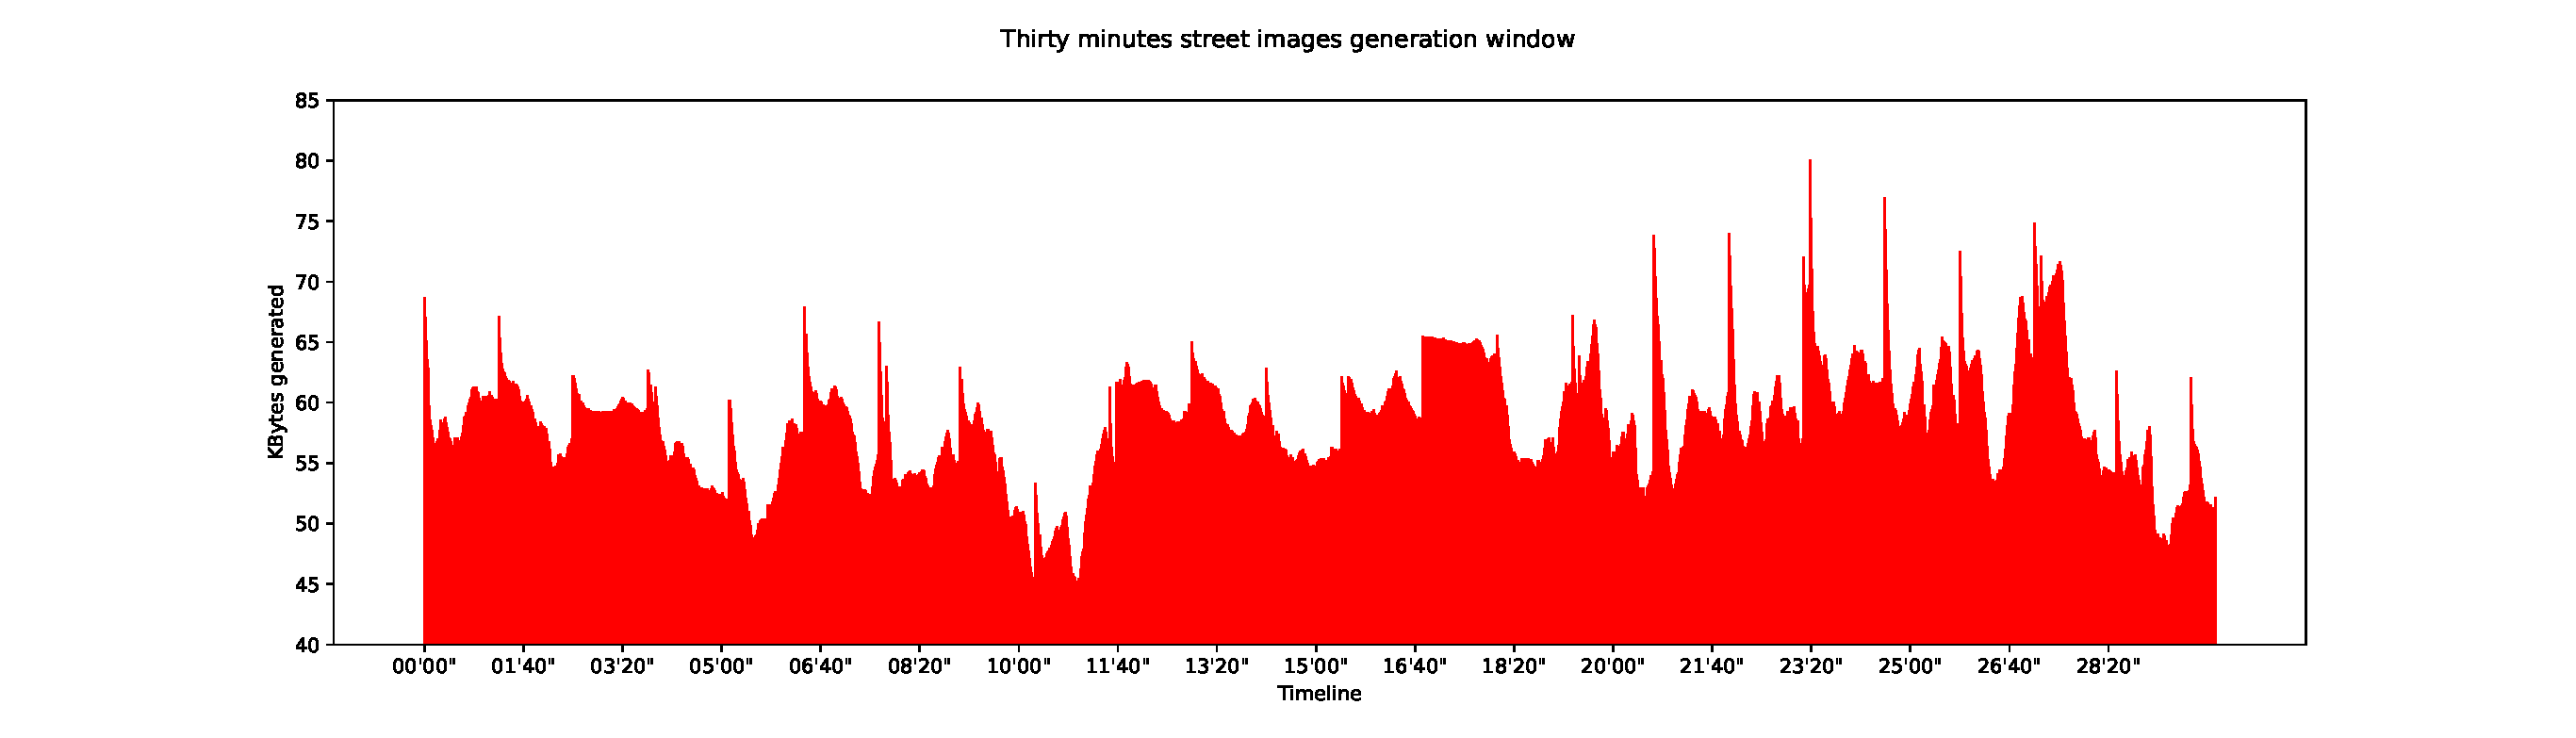
\includegraphics[clip,scale=0.3]{figures/dogs_finder_stream_exerpt}
\par\end{centering}
}\subfloat[street image example\label{fig:street-image-example}]{\includegraphics[scale=0.25]{figures/cycling\lyxdot 2130}

}\\
\subfloat[Cow images stream\label{fig:Cow-images-stream}]{\begin{centering}
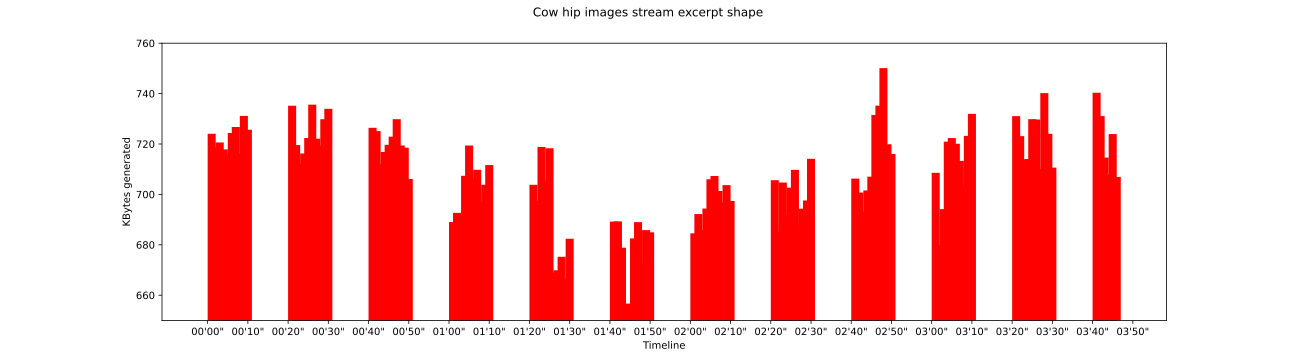
\includegraphics[clip,scale=0.3]{figures/cow_bcs_stream_exerpt}
\par\end{centering}
}\subfloat[Cow image example\label{fig:Cow-image-example}]{\includegraphics[scale=0.2]{figures/cow_images\lyxdot 84}

}\\
\subfloat[Foot images stream\label{fig:Foot-images-stream}]{\begin{centering}
\includegraphics[clip,scale=0.3]{figures/diabetes_stream_exerpt}
\par\end{centering}
}\subfloat[Foot image example\label{fig:Foot-image-example}]{\includegraphics[clip,scale=0.1]{figures/diabetes\lyxdot 157}

}

\caption{Dew computing streams examples}
\end{figure}

Irrespective of the application domain, the three examples represent
streams with different characteristics not only by the dynamics of
input image generation but also the computing power required to perform
inferences. In addition, it is assumed that inferences results should
be available at the master node with minimun delay, i.e., as close
as possible to a real time detection, which is a characteristic of
computing services provided at edge.

\subsection{Results}

\begin{table}
\begin{centering}
\begin{tabular}{cccc}
\toprule 
Edge Node & Load Balancing & Makespan (mins) & Jain's Fairness Index\tabularnewline
\midrule
\midrule 
Raspberry pi 4 & N/A & 63.2 & N/A\tabularnewline
\midrule 
Jetson Nano & N/A & 34.27 & N/A\tabularnewline
\midrule 
Gigabyte Brix & N/A & \textbf{30.14} & N/A\tabularnewline
\midrule 
\multirow{2}{*}{Cluster 202} & Round Robin & 45.28 & 0.925\tabularnewline
\cmidrule{2-4} \cmidrule{3-4} \cmidrule{4-4} 
 & Pull Based & 44.66 & 0.925\tabularnewline
\midrule 
\multirow{2}{*}{Cluster 302} & Round Robin & 41.53 & 0.933\tabularnewline
\cmidrule{2-4} \cmidrule{3-4} \cmidrule{4-4} 
 & Pull Based & 32.34 & 0.96\tabularnewline
\midrule 
\multirow{2}{*}{Cluster 301} & Round Robin & 30.76 & 0.96\tabularnewline
\cmidrule{2-4} \cmidrule{3-4} \cmidrule{4-4} 
 & Pull Based & 30.42 & 0.896\tabularnewline
\midrule 
\multirow{2}{*}{Cluster 408} & Round Robin & 30.41 & 0.907\tabularnewline
\cmidrule{2-4} \cmidrule{3-4} \cmidrule{4-4} 
 & Pull Based & 30.24 & 0.818\tabularnewline
\bottomrule
\end{tabular}
\par\end{centering}
\caption{Sense while travel scenario (30 minutes stream)}

\end{table}

\begin{table}
\begin{centering}
\begin{tabular}{cccc}
\toprule 
Edge Node & Load Balancing & Makespan (mins) & Jain's Fairness Index\tabularnewline
\midrule
\midrule 
Raspberry pi 4 & N/A & 26.92 & N/A\tabularnewline
\midrule 
Jetson Nano & N/A &  & N/A\tabularnewline
\midrule 
Gigabyte Brix & N/A & \textbf{3.9} & N/A\tabularnewline
\midrule 
\multirow{2}{*}{Cluster 304} & Round Robin & 6.81 & 0.667\tabularnewline
\cmidrule{2-4} \cmidrule{3-4} \cmidrule{4-4} 
 & Pull Based & 4.96 & 0.926\tabularnewline
\midrule 
\multirow{2}{*}{Cluster 409} & Round Robin & 5.06 & 0.75\tabularnewline
\cmidrule{2-4} \cmidrule{3-4} \cmidrule{4-4} 
 & Pull Based & 3.96 & 0.75\tabularnewline
\bottomrule
\end{tabular}
\par\end{centering}
\caption{Body Condition Score scenario (03:50 minutes stream)}
\end{table}
\begin{table}
\begin{centering}
\begin{tabular}{cccc}
\toprule 
Edge Node & Load Balancing & Makespan (mins) & Jain's Fairness Index\tabularnewline
\midrule
\midrule 
Raspberry pi 4 & N/A & 27.72 & N/A\tabularnewline
\midrule 
Jetson Nano & N/A &  & N/A\tabularnewline
\midrule 
Gigabyte Brix & N/A & \textbf{8.99} & N/A\tabularnewline
\midrule 
\multirow{2}{*}{Cluster 411} & Round Robin & 25.24 & 0.833\tabularnewline
\cmidrule{2-4} \cmidrule{3-4} \cmidrule{4-4} 
 & Pull Based & 9.34 & 0.643\tabularnewline
\bottomrule
\end{tabular}
\par\end{centering}
\caption{E-health early detection scenario (08:55 minutes stream)}
\end{table}


\section{Conclusions and Future works}
\begin{itemize}
\item Concluir sobre la factibilidad de llevar a cabo un sistema para inferencia
en el edge empleando poder c�mputo aportado dispositivos m�viles compar�ndolo
con lo que podr�a ser el uso de un nodo fijo de prop�sito espec�fico.
\item Presentar como futura l�nea de trabajo la posibilidad de que utilizar
un modelo de paralelismo/distribuci�n de la inferencia donde cada
nodo es encargado de todas las inferencias pero de pocas capas de
la arquitectura DNN, es decir, mantener distribuida la arquitectura
de capas. 
\end{itemize}
\bibliographystyle{plain}
\bibliography{references}

\end{document}
